\chapter{Diffusion Models}

By 2019, GANs had become incredibly powerful. Models like StyleGAN could generate faces so realistic that people often couldn't tell they were fake.
Researchers believed GANs might become the future of Image Generation. But despite their impressive results, one major problem remained: Training a GAN was still difficult.
Even after years of improvements (DCGAN, WGAN, StyleGAN, BigGAN...) GANs still suffered from several issues:
\begin{itemize}
    \item \textbf{Training instability} because the Generator and Discriminator constantly compete
    \item \textbf{Mode collapse}: where the Generator produces limited varieties of images
    \item \textbf{Sensitive hyperparameters}: making training difficult to reproduce
    \item \textbf{Balancing two networks is challenging}: if one becomes too strong, the other stops learning.
\end{itemize}

Researchers wanted a model that was:
\begin{itemize}
    \item easier to train
    \item more stable
    \item capable of producing diverse, high-quality images
\end{itemize}

Instead of asking: ``Can one network fool another network?'' \\
Researchers asked: ``Can we learn how to remove noise from an image?''

This question completely changed the direction of generative modeling. There would be:
\begin{itemize}
    \item no Generator vs Discriminator
    \item no adversarial game
    \item no competition
\end{itemize}
Instead, the model would learn a much simpler task: \textbf{Denoising}.

The brilliant idea behind diffusion models is to reverse the process of adding noise. Since gradually corrupting an image with Gaussian noise is simple and predictable, researchers realized that a neural network could be trained to learn the opposite process. Instead of generating an image directly, the model starts from pure random noise and removes a small amount of noise at each step, gradually reconstructing a realistic image. This transforms image generation into a sequence of simple denoising steps, making the learning process much more stable than the adversarial training used in GANs.

\subsection*{Why is This Easier Than GANs?}

Unlike GANs, where the Generator and Discriminator compete and the learning objective constantly changes, diffusion models train a single neural network with one fixed objective: predict and remove a small amount of noise. This stable objective makes diffusion models much easier to train.

\begin{itemize}
    \item Diffusion models do not learn to generate an image directly. Instead, they learn: \textbf{How To Remove a very small amount of Noise at each step.}
\end{itemize}

Diffusion models quickly became the dominant generative approach because they offered several advantages:
\begin{itemize}
    \item More stable training than GANs.
    \item Better diversity (less mode collapse).
    \item Excellent image quality.
    \item Easy to condition on text, segmentation maps, depth maps, or other inputs.
    \item Flexible enough for tasks like image editing, inpainting, and super-resolution.
\end{itemize}

\textbf{The main drawback} is that image generation is slower, since it requires many denoising steps.

\section{Core Principles of Diffusion}

Diffusion models were created to overcome the instability of GANs. Instead of training two competing networks, they train a single neural network to solve a simple and stable task: \textbf{Predict and Remove noise}.
\begin{itemize}
    \item \textbf{The Forward Process} gradually destroys an image by adding Gaussian noise until only random noise remains.
    \item \textbf{The Reverse Process} learns to remove that noise step by step, eventually reconstructing a realistic image. This simple idea became the foundation of modern image generation systems such as Stable Diffusion.
\end{itemize}

\subsection*{I) The Forward Diffusion Process}

The forward diffusion process gradually adds Gaussian noise to a clean image until it becomes pure random noise:
\begin{itemize}
    \item No neural network
    \item No learning
    \item Fixed corruption process
\end{itemize}

\textbf{Forward Process: starting from a clean image $x_0$:}
\[
x_0 \longrightarrow x_1 \longrightarrow x_2 \longrightarrow x_3 \longrightarrow x_4 \longrightarrow x_5 \dots \longrightarrow x_t
\]
Each step adds a small amount of Gaussian noise, making the image progressively noiser.

Adding all the noise at once would completely destroy the image and make it impossible to learn the reverse process.
By adding small amounts of noise at each step, the model only needs to learn how to reverse small changes, which is much easier.

\subsection*{Gaussian Noise}

The added noise is sampled from a standard Gaussian distribution:
\[
\epsilon \sim \mathcal{N}(0, 1)
\]
where:
\[
\text{Mean} = 0, \quad \text{Variance} = 1
\]
Each pixel receives a small random value sampled from this distribution. For example:
\[
\text{pixel} = 120, \quad \text{Noise} = +2 \quad \rightsquigarrow \quad \text{pixel} = 122
\]
or:
\[
\text{pixel} = 120, \quad \text{Noise} = -3 \quad \rightsquigarrow \quad \text{pixel} = 117
\]
Every pixel gets a different random value.

The forward process is a \textbf{Markov chain}. This means: each step depends only on the previous step, not on the entire history. For example:
\[
x_0 \longrightarrow x_1 \longrightarrow x_2 \longrightarrow x_3
\]
To compute $x_3$ we only need $x_2$; we do not need $x_0$ or $x_1$.

\subsection*{The Noise Schedule}

We don't add a random amount of noise each step. Instead, we define a noise schedule:
\begin{align*}
\text{step 1} &\longrightarrow 0.1\% \text{ noise} \\
\text{step 2} &\longrightarrow 0.2\% \text{ noise} \\
&\vdots \\
\text{step 1000} &\longrightarrow \text{Very noisy}
\end{align*}

The schedule controls how much noise is added at every step. Different schedules affect image quality and sampling speed.

After many diffusion steps, every image converges to the same distribution:
\[
x_T \sim \mathcal{N}(0, I)
\]
Regardless of whether the original image is a cat, car, house... it eventually becomes pure Gaussian noise.

Since every image eventually becomes Gaussian noise, generation becomes simple:
\begin{enumerate}
    \item Sample random noise $\sim \mathcal{N}(0, 1)$
    \item Learn how to reverse the diffusion
    \item Recover a realistic image
\end{enumerate}
Instead of learning to generate an image from scratch, the model only learns to remove noise little by little.

\subsection*{II) Reverse Diffusion}

After the forward process, the image becomes pure Gaussian noise $x_T$. The original image cannot be recovered directly because the information has been destroyed. Instead, the model must learn how to gradually remove the noise.

The reverse process performs the opposite of forward diffusion:
\[
\text{Pure noise} \longrightarrow \text{Less noise} \longrightarrow \text{Cleaner Image} \longrightarrow \dots \longrightarrow \text{Final Image}
\]
Instead of generating an image in one step, it is reconstructed progressively.

The diffusion model receives $(\text{Noisy Image}, \text{Time Step } t)$ and predicts: \textbf{Predicted Noise} ($\epsilon$). The network doesn't predict the clean image, it predicts the noise contained in the image.
Predicting the added Gaussian noise is simpler and more stable than predicting the clean image directly.

Once the noise is estimated:
\[
\text{Cleaner Image} = \text{Noisy Image} - \text{Predicted Noise}
\]
This process is repeated many times until a clean image is obtained.

\subsection*{Time Step Embedding}

The same noisy image may require different amounts of denoising depending on how much noise was originally added.
The time step $t$ tells the network:
\begin{itemize}
    \item how noisy the image is
    \item how much noise should be removed
\end{itemize}
Without $t$, the network would not know the current stage of the diffusion process.

\subsection*{Training Process}

For each training image:
\begin{enumerate}
    \item Start with a clean image $x_0$
    \item Randomly choose a time step $t$
    \item Add the corresponding Gaussian noise
    \item Feed $(\text{Noisy Image}, t)$ into the network
    \item Train the network to predict the true added noise using MSE Loss.
\end{enumerate}

\subsection*{Inference (Image Generation)}

During generation:
\begin{enumerate}
    \item Sample random Gaussian noise $x_T \sim \mathcal{N}(0, I)$
    \item Predict the noise
    \item Remove the predicted noise
    \item Repeat for all time steps until reaching $x_0$.
\end{enumerate}

\begin{figure}[H]
\centering
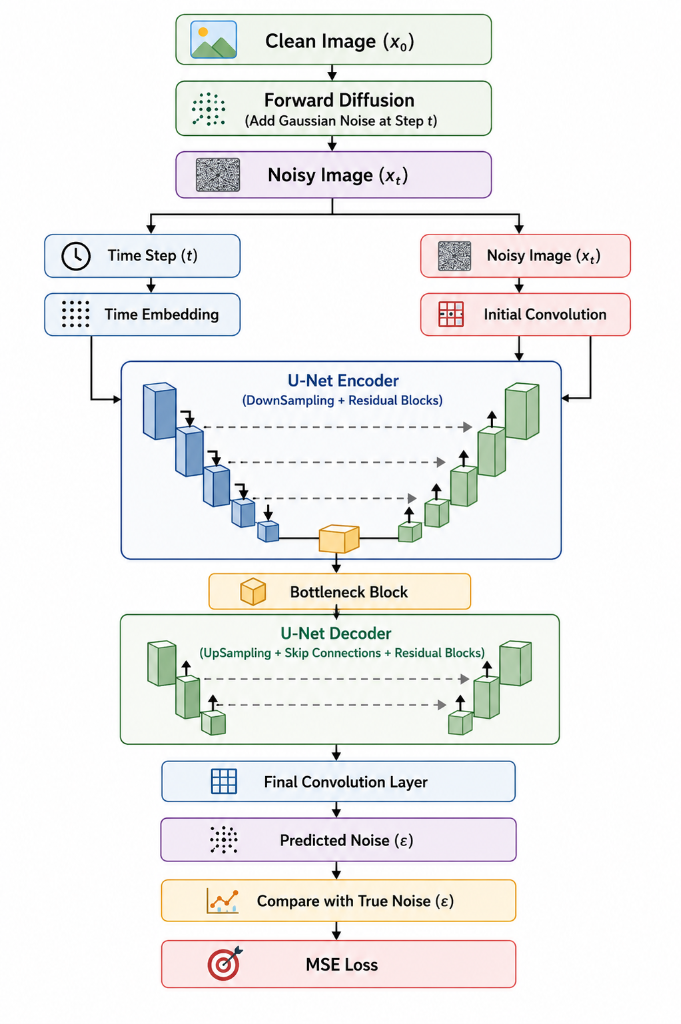
\includegraphics[width=0.88\textwidth]{figures/fig_10_1_diffusion_training_pipeline.png}
\caption{Diffusion Model Training and Noise Prediction Pipeline.}
\label{fig:diffusion_training_pipeline}
\end{figure}

\subsection*{Diffusion More Stable Than GANs}

\textbf{GAN:}
\begin{itemize}
    \item Two competing networks (Generator vs Discriminator)
    \item The objective changes during training
    \item Training can become unstable
\end{itemize}

\textbf{Diffusion:}
\begin{itemize}
    \item Only one neural network
    \item One fixed objective: predict the added noise
    \item Stable optimization using a simple MSE loss
\end{itemize}

\textbf{Summary:} The reverse diffusion process is the learned part of a diffusion model. Starting from pure Gaussian noise, a neural network repeatedly predicts the noise present in the current image and removes a small portion of it at each step. During training, the model receives a noisy image together with its time step and learns to predict the exact Gaussian noise that was added using an MSE loss. During inference, the same denoising process is applied iteratively to random noise until a realistic image is generated. Predicting noise instead of directly predicting the clean image is one of the key ideas that makes diffusion models stable and effective.

\section{DDPM (Denoising Diffusion Probabilistic Models)}

DDPM is the first practical diffusion model. It uses a U-Net to learn how to remove Gaussian noise from an image step by step until a clean image is reconstructed.
U-Net is well suited for this task because denoising is an image-to-image problem: the input is a noisy image and the output is a predicted noise map of the same size. Its encoder extracts high-level features, while the decoder reconstructs fine image details with the help of skip connections, enabling accurate denoising at every diffusion step.



\begin{figure}[H]
\centering
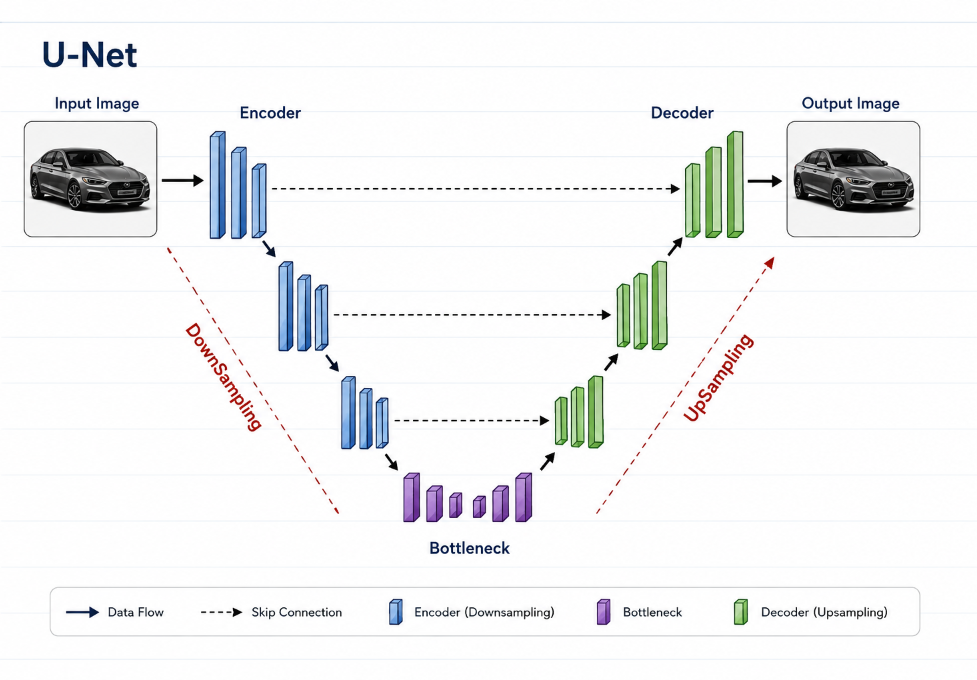
\includegraphics[width=0.88\textwidth]{figures/fig_10_2_unet_overview.png}
\caption{U-Net Architecture Overview for Image-to-Image Denoising.}
\label{fig:unet_overview}
\end{figure}

\begin{itemize}
    \item It was originally designed for image segmentation.
    \item Denoising is also an image-to-image problem.
\end{itemize}
Since both input and output are images of the same size, U-Net is an excellent choice.

\begin{figure}[H]
\centering
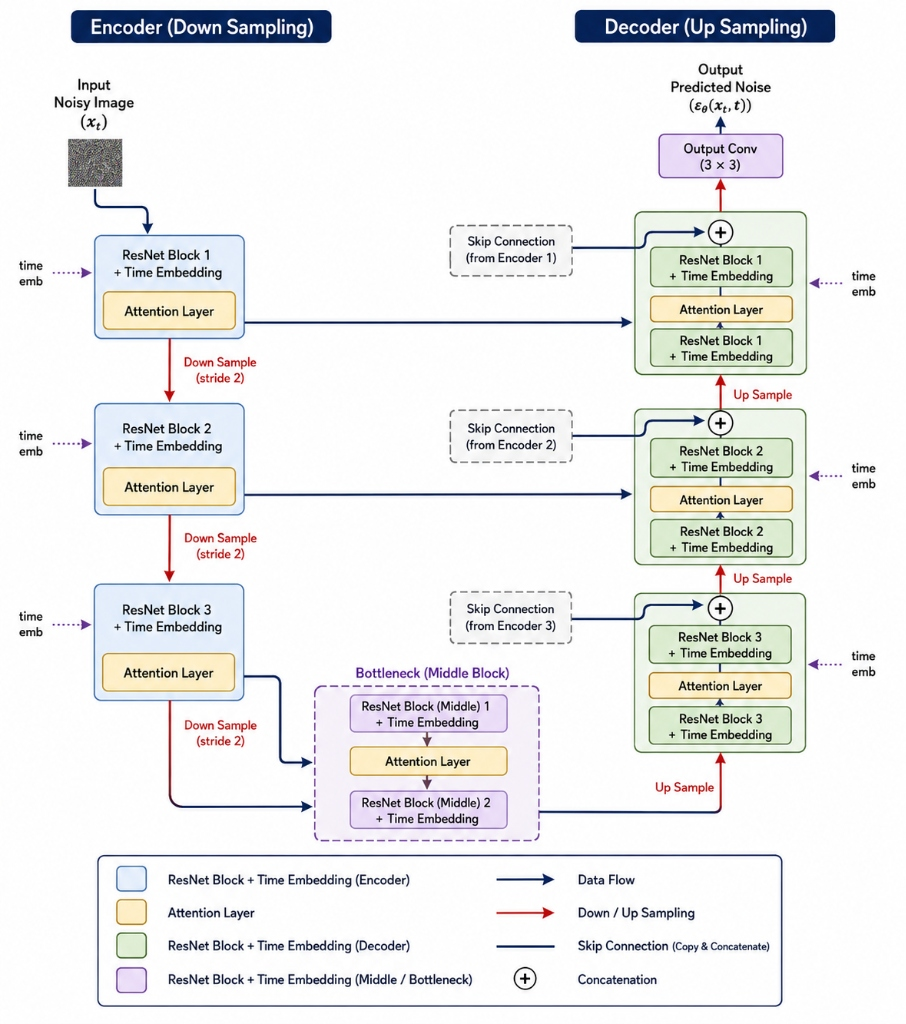
\includegraphics[width=0.95\textwidth]{figures/fig_10_3_ddpm_unet_detailed.jpg}
\caption{Detailed DDPM U-Net Architecture with ResNet Blocks, Attention Layers, and Time Embeddings.}
\label{fig:ddpm_unet_detailed}
\end{figure}

\begin{figure}[H]
\centering
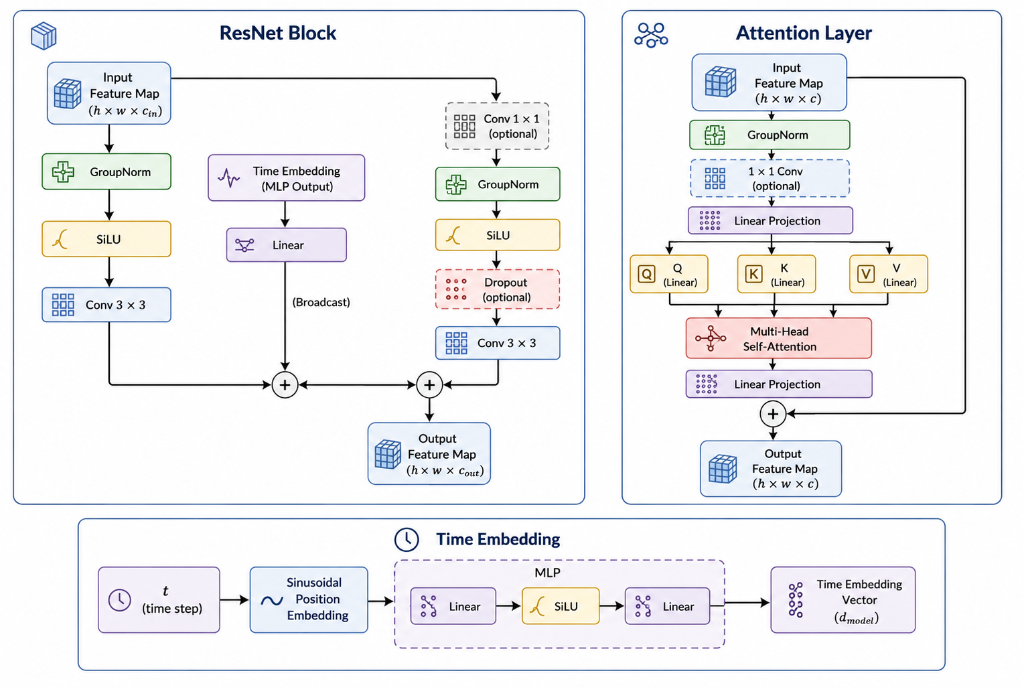
\includegraphics[width=0.95\textwidth]{figures/fig_10_4_unet_internal_components.png}
\caption{Internal Building Blocks of the DDPM U-Net: ResNet Block, Attention Layer, and Time Embedding MLP.}
\label{fig:unet_internal_components}
\end{figure}

\subsection*{Time Embedding Integration}

The U-Net receives two inputs:
\begin{itemize}
    \item Noisy image $x_t$
    \item Time step $t$
\end{itemize}

The integer $t$ is converted into a time embedding vector. This embedding is injected into multiple residual blocks so the network knows how much denoising to perform.

\subsection*{Training Process Step-by-Step}

\begin{enumerate}
    \item Select a clean image $x_0$
    \item Randomly choose a timestep $t$
    \item Add Gaussian noise to obtain $x_t$
    \item Feed $(x_t, t)$ into the U-Net
    \item Predict the added noise $\hat{\epsilon}$
    \item Compute the Loss $L_{\text{MSE}} = \|\epsilon - \hat{\epsilon}\|^2$
    \item Update the U-Net using backpropagation
\end{enumerate}

\begin{figure}[H]
\centering
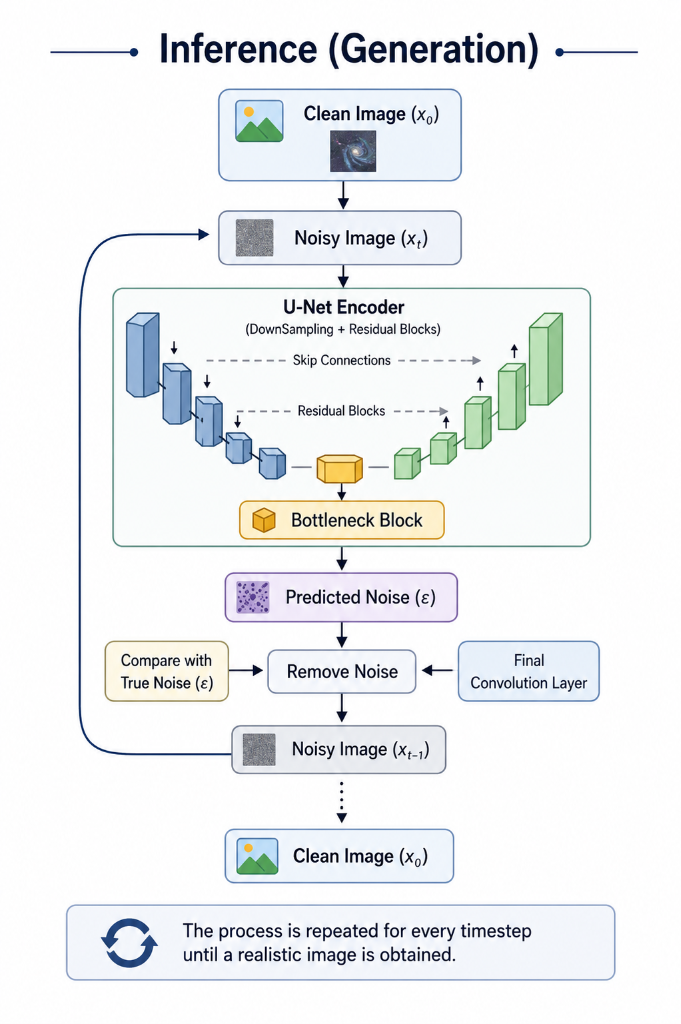
\includegraphics[width=0.88\textwidth]{figures/fig_10_5_diffusion_inference_pipeline.png}
\caption{Inference (Generation) Denoising Loop in Diffusion Models.}
\label{fig:diffusion_inference_pipeline}
\end{figure}

\section{Classifier-Free Guidance (CFG)}

\subsection*{I) Guidance}

Without additional information, diffusion models generate random images. To generate a specific object or scene, the model needs guidance.

\textbf{The Main Idea of Classifier Guidance is using two models:}
\begin{itemize}
    \item Diffusion model
    \item External image classifier
\end{itemize}
The classifier provides gradients that push the generated image toward the desired class.

\textbf{Limitation:}
\begin{itemize}
    \item Requires training an additional classifier
    \item More computationally expensive
\end{itemize}

\subsection*{II) Classifier-Free Guidance (CFG)}

Instead of using an external classifier, the diffusion model learns both:
\begin{itemize}
    \item \textbf{Conditional Generation}: Noise + Prompt
    \item \textbf{Unconditional Generation}: Noise only
\end{itemize}

During training, the conditioning information (text/class) is randomly removed, allowing one model to learn both behaviors.

\subsection*{CFG During Inference}

During inference, the model performs two noise predictions:
\begin{enumerate}
    \item \textbf{Unconditional prediction}: Noise only ($\hat{\epsilon}_{\text{uncond}}$)
    \item \textbf{Conditional prediction}: Noise + Prompt ($\hat{\epsilon}_{\text{cond}}$)
\end{enumerate}
They are combined using:
\[
\hat{\epsilon}_{\text{CFG}} = \hat{\epsilon}_{\text{uncond}} + w \cdot (\hat{\epsilon}_{\text{cond}} - \hat{\epsilon}_{\text{uncond}})
\]
where $w = \text{Guidance Scale}$: Controls how strongly the prompt influences the generated image.
\begin{itemize}
    \item \textbf{Low scale}: More creative, weaker adherence to the prompt
    \item \textbf{High scale}: Follows the prompt more closely
\end{itemize}
Typically values for CFG scale are $7 - 8$.

Today, almost every text-to-image diffusion model uses Classifier-Free Guidance.
Examples:
\begin{itemize}
    \item Stable Diffusion
    \item SDXL
    \item FLUX
    \item Many modern diffusion models
\end{itemize}
because it:
\begin{itemize}
    \item requires no extra classifier
    \item is simple
    \item gives users control over prompt strength.
\end{itemize}

\begin{figure}[H]
\centering
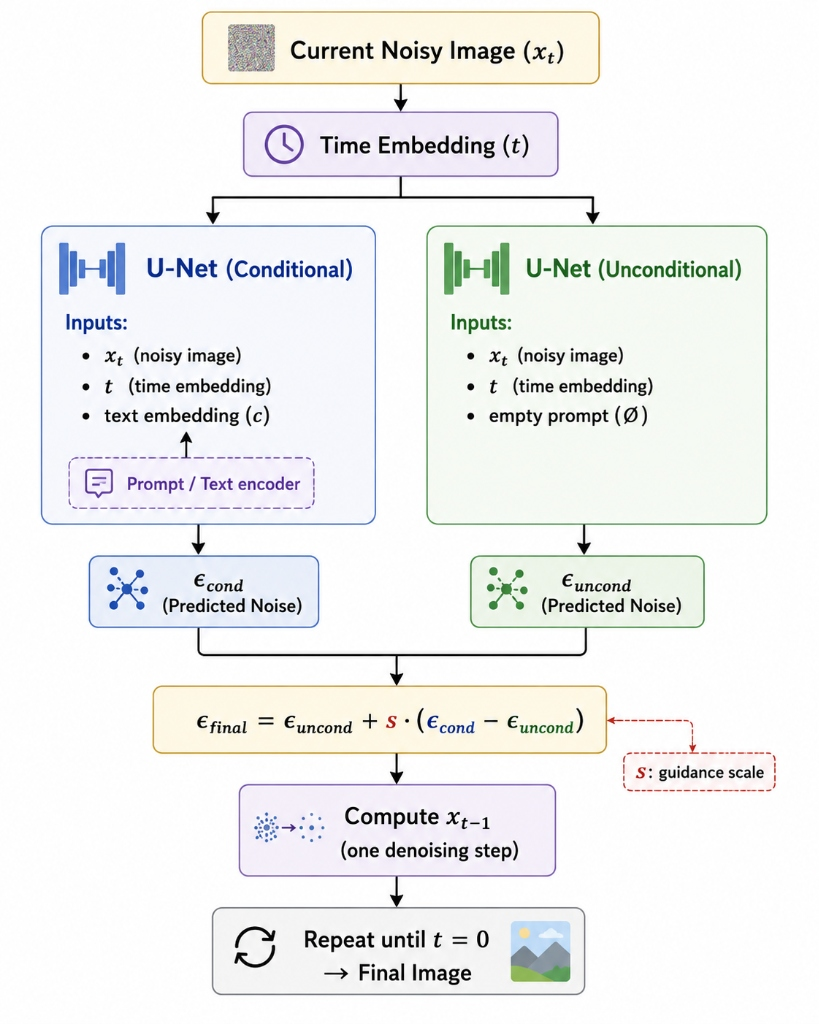
\includegraphics[width=0.88\textwidth]{figures/fig_10_6_classifier_free_guidance.jpg}
\caption{Classifier-Free Guidance (CFG) Denoising Pipeline.}
\label{fig:classifier_free_guidance}
\end{figure}

\section{Latent Diffusion Models (LDM)}

DDPM and DDIM perform diffusion directly on pixels.
For example, suppose we have a $512 \times 512$ RGB image:
\[
512 \times 512 \times 3 \longrightarrow 786,432 \text{ values}
\]
At every denoising step, the U-Net processes all 786,432 pixel values. For 1,000 denoising steps, this requires an enormous amount of computation and memory.
Researchers asked: ``Do we really need to diffuse millions of pixels?''

The main idea of LDM is to use a Variational Autoencoder (VAE) to compress an image into a much smaller latent representation before diffusion.
The diffusion model never operates on the original image; it works entirely in the latent space.

\begin{figure}[H]
\centering
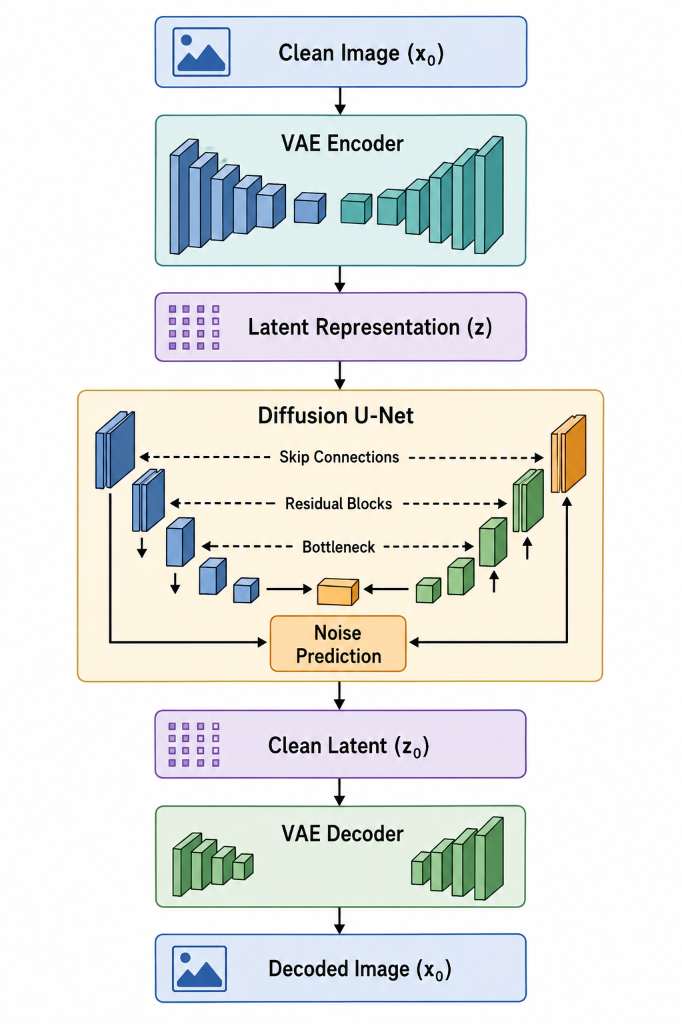
\includegraphics[width=0.75\textwidth]{figures/fig_10_7_latent_diffusion_architecture.png}
\caption{Latent Diffusion Model Architecture.}
\label{fig:latent_diffusion_architecture}
\end{figure}

LDM models are much faster because the latent diffusion process is performed on a compressed representation instead of raw pixels.
The VAE encoder compresses a high-resolution image into a much smaller representation, reducing the amount of data processed by the U-Net at every denoising step.

For example, a $512 \times 512 \times 3$ image ($786,432$ values) is compressed into a $64 \times 64 \times 4$ latent representation ($16,384$ values), meaning the model processes about $48\times$ fewer values.
This drastically reduces both computational cost and memory usage while maintaining high image quality, making image generation dramatically faster.

The VAE compresses the image while preserving key semantic information (objects, colors, textures) and removing unnecessary details (such as exact pixel noise). This allows the diffusion model to focus on high-level image generation instead of low-level pixel noise.

\begin{figure}[H]
\centering
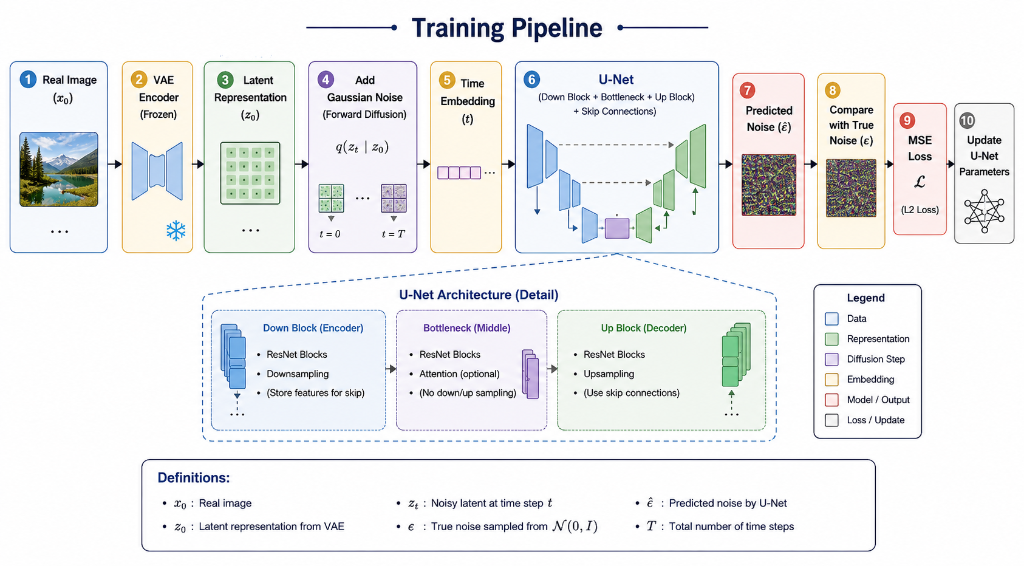
\includegraphics[width=0.95\textwidth]{figures/fig_10_8_ldm_training_pipeline.png}
\caption{Training Pipeline for Latent Diffusion Models.}
\label{fig:ldm_training_pipeline}
\end{figure}

\begin{figure}[H]
\centering
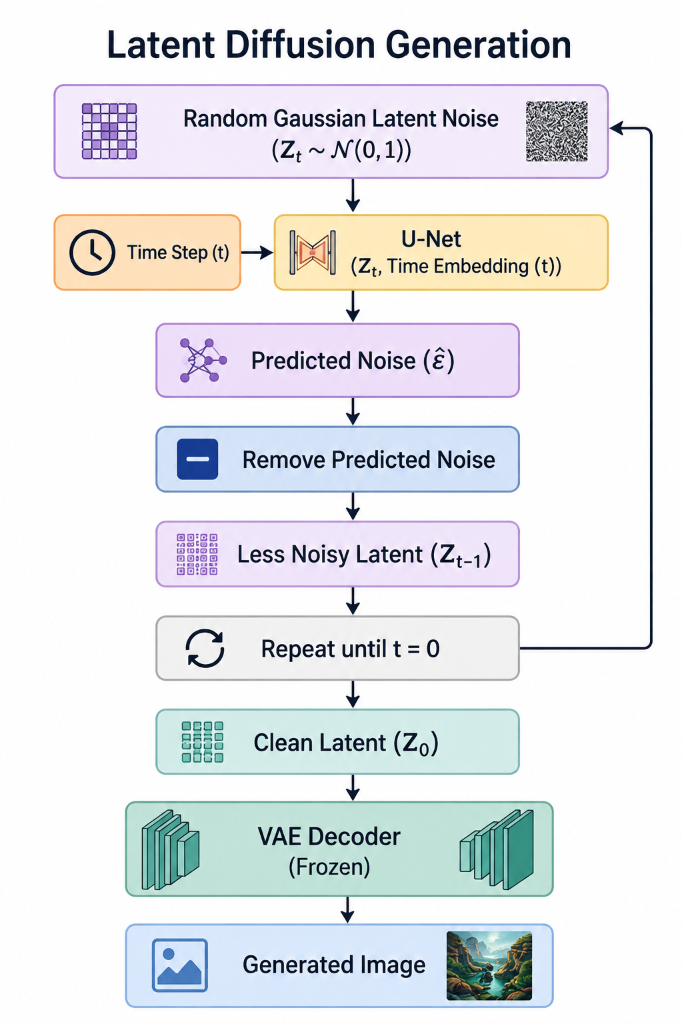
\includegraphics[width=0.75\textwidth]{figures/fig_10_9_ldm_generation_pipeline.png}
\caption{Latent Diffusion Generation and Inference Pipeline.}
\label{fig:ldm_generation_pipeline}
\end{figure}

\subsection*{Advantages of LDM}
\begin{itemize}
    \item Uses much less GPU memory
    \item Faster training and generation
    \item Supports high-resolution image generation
    \item Maintains excellent image quality
\end{itemize}

\subsection*{Drawbacks}
\begin{itemize}
    \item Image quality depends on the VAE compression quality (if information is lost during compression, it cannot be recovered)
    \item The system requires two models: VAE and Diffusion Model.
\end{itemize}

\section{Stable Diffusion}

Stable Diffusion is a Latent Diffusion Model (LDM) that can generate images directly from text prompts.
It combines:
\begin{itemize}
    \item \textbf{VAE}: Compresses and reconstructs images
    \item \textbf{Diffusion Model (U-Net)}: Denoises the latent representation
    \item \textbf{CLIP Text Encoder}: Converts text prompts into numerical text embeddings that the diffusion model can understand
    \item \textbf{Cross-Attention}: Connects the text embeddings with the image generation process
    \item \textbf{CFG (Classifier-Free Guidance)}: Controls how strongly the generated image follows the prompt.
\end{itemize}

\begin{figure}[H]
\centering
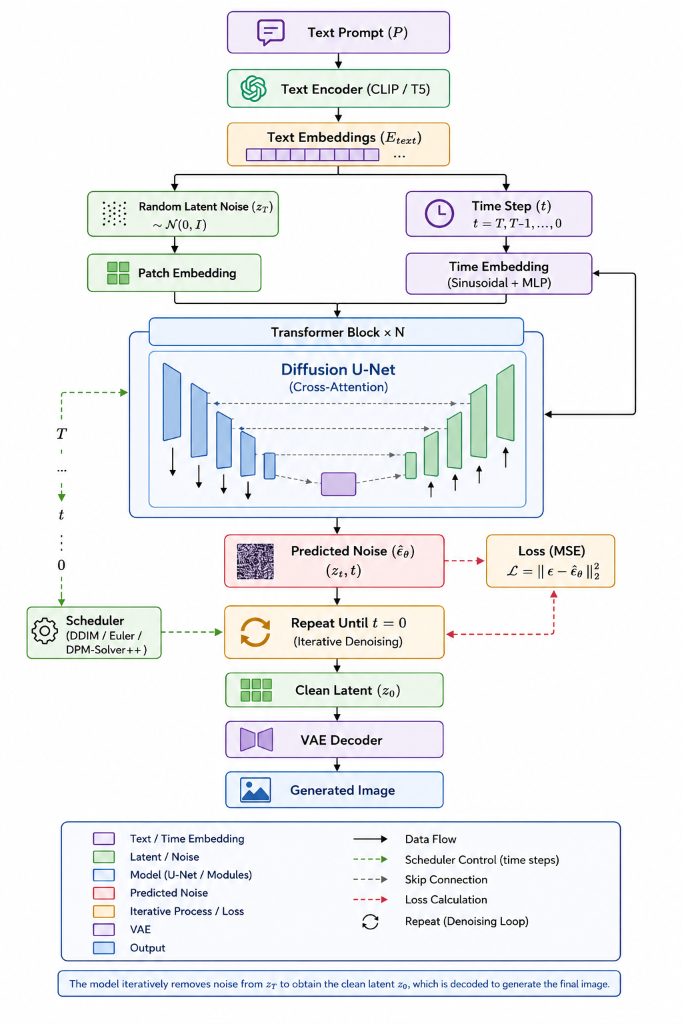
\includegraphics[width=0.95\textwidth]{figures/fig_10_10_conditioning_mechanisms.png}
\caption{Conditioning Mechanisms in Latent Diffusion Models.}
\label{fig:conditioning_mechanisms}
\end{figure}

In the standard classifier-free guidance (CFG) mechanism, the denoiser performs two noise predictions at each denoising step:

\begin{enumerate}
    \item A prediction without the text prompt (unconditional prediction).
    \item A prediction conditioned on the text prompt (conditional prediction).
\end{enumerate}

These two predictions are combined using \textbf{Classifier-Free Guidance (CFG)} to produce the final noise estimate for that denoising step. Other diffusion systems may use different conditioning or guidance mechanisms.

Stable Diffusion became extremely popular and revolutionary because it:

\begin{itemize}
    \item Generates high-quality images.
    \item Runs efficiently on consumer GPUs.
    \item Supports text-to-image generation.
    \item Uses Classifier-Free Guidance (CFG) to improve prompt adherence.
    \item Can be fine-tuned on new styles and concepts (e.g., LoRA and ControlNet).
    \item Has a large open-source ecosystem of models, tools, and extensions.
\end{itemize}

\section{Diffusion Transformers (DiT)}

Diffusion Transformers are a family of diffusion-model architectures that use a Vision Transformer (ViT)-style backbone instead of a U-Net.
The noisy latent is split into patches, converted into tokens, and processed with Transformer blocks to predict the noise.

DiT changes the denoising backbone; its latent representation, conditioning, guidance, and training design depend on the specific diffusion system.

\subsection*{Why Replace U-Net?}
\begin{itemize}
    \item U-Net relies on Convolutions, which mainly focus on local features.
    \item Transformers use Self-Attention, allowing every patch to interact with every other patch.
    \item Transformers scale much better as dataset size, compute, and model parameters increase.
\end{itemize}

\begin{figure}[H]
\centering
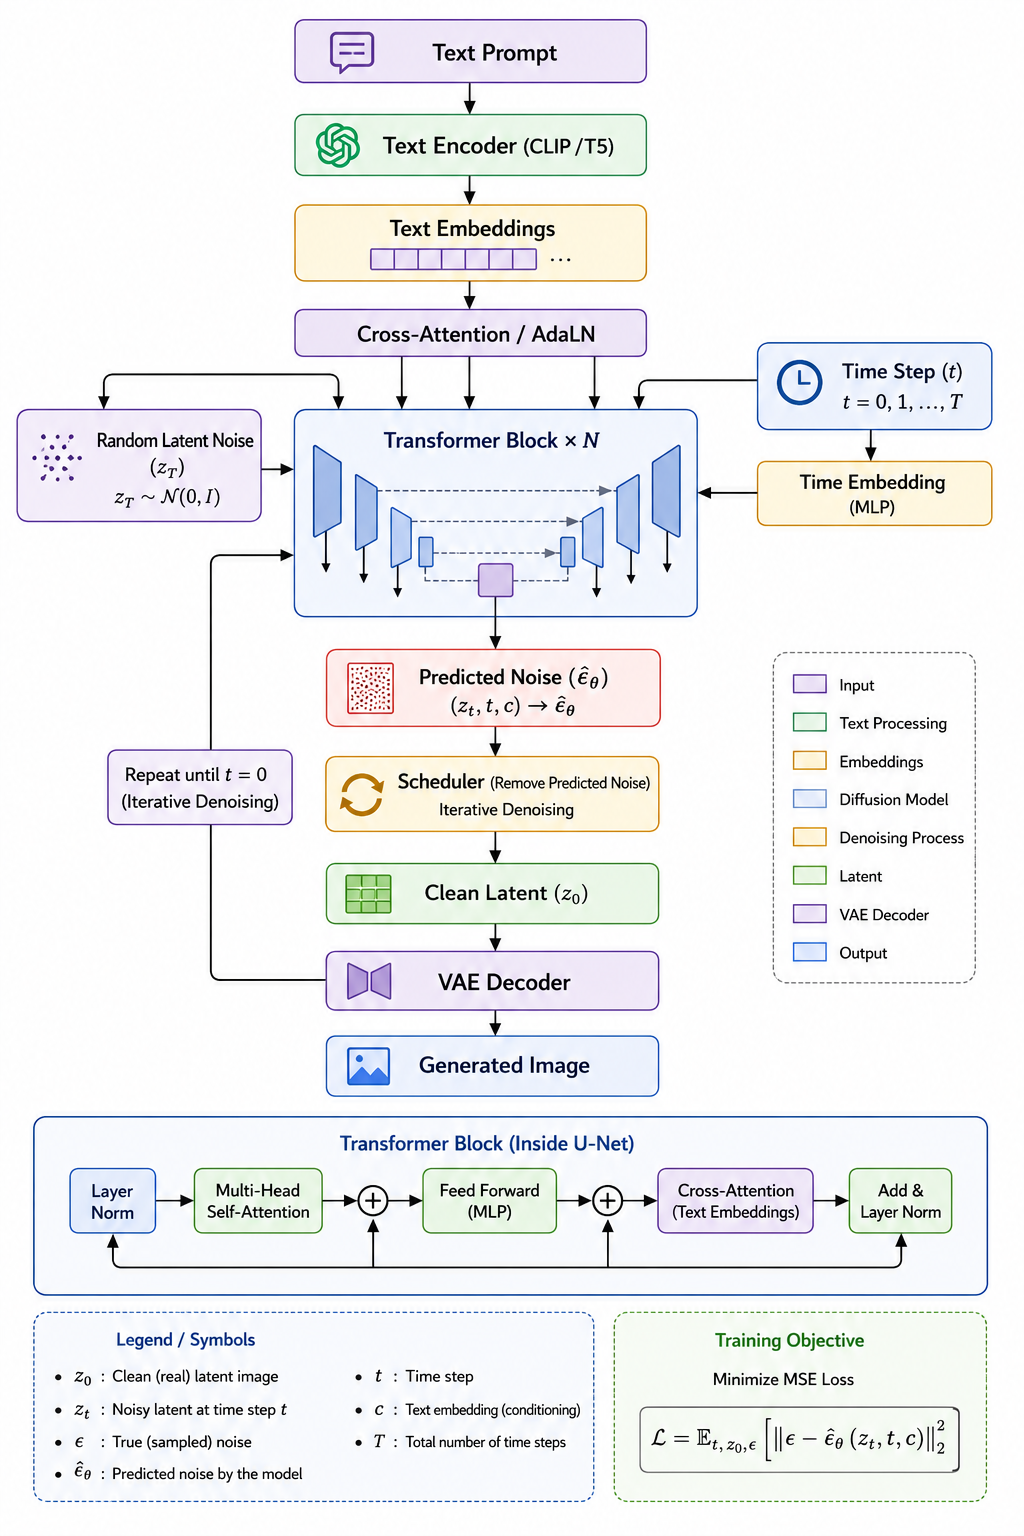
\includegraphics[width=0.95\textwidth]{figures/ChatGPT Image Aug 5, 2026, 03_19_00 AM.png}
\caption{Diffusion Transformer (DiT) Architecture Details.}
\label{fig:dit_architecture}
\end{figure}

\section{DiT Conditioning and Adaptive Layer Normalization}

A Diffusion Transformer (DiT) uses a Vision Transformer (ViT)-style architecture as its denoising backbone. In the original DiT design, the noisy latent produced by the VAE is divided into small patches, which are converted into latent patch tokens and processed by a stack of Transformer blocks.

Unlike a standard Vision Transformer, DiT must also receive the conditioning information required by the diffusion process. Each Transformer block therefore combines three sources of information:

\begin{enumerate}
    \item \textbf{Latent patch tokens}, obtained from the noisy latent representation.
    \item \textbf{Time embedding}, which indicates the current diffusion step $t$, allowing the model to know where it is in the denoising process.
    \item \textbf{Text embedding}, generated by a text encoder from the input prompt, providing semantic guidance for image generation.
\end{enumerate}

Rather than injecting the time and text embeddings through convolutional blocks as in U-Net-based diffusion models, DiT incorporates this conditioning information into every Transformer block using \textbf{Adaptive Layer Normalization (AdaLN)}:

\[
\text{AdaLN}(x,t,c)=\gamma(t,c)\,\text{LN}(x)+\beta(t,c),
\]

where $x$ represents the Transformer token features, $\text{LN}(\cdot)$ denotes Layer Normalization, and $\gamma(t,c)$ and $\beta(t,c)$ are learned scale and shift parameters generated from the time-step and text-conditioning embeddings. Consequently, every Transformer block is aware of both the current diffusion step and the prompt being followed, enabling the model to adapt its feature activations throughout the denoising process.

By leveraging global self-attention and the excellent scaling properties of Transformers, DiT has become one of the leading architectures for modern diffusion models. As the model size, training dataset, and computational resources increase, its image generation quality continues to improve, making Transformer-based diffusion models highly scalable.

\section{SDXL (Stable Diffusion XL)}

SDXL is an improved version of Stable Diffusion that significantly increases model capacity while preserving the original latent diffusion framework. Rather than introducing a completely new architecture, SDXL retains the same fundamental components, including the Variational Autoencoder (VAE), latent diffusion process, U-Net denoiser, and Classifier-Free Guidance (CFG), while incorporating several important enhancements.

The main improvements of SDXL include:

\begin{itemize}
    \item A larger and more expressive U-Net architecture.
    \item Dual text encoders (CLIP ViT-L and OpenCLIP ViT-bigG), enabling richer prompt understanding.
    \item Improved image quality and native high-resolution image generation at $1024 \times 1024$ pixels.
\end{itemize}
\section{FLUX}

FLUX (2024) is a modern text-to-image model developed by Black Forest Labs.
Instead of the traditional U-Net, FLUX uses a Transformer-based backbone (similar in spirit to DiT).

Key improvements:
\begin{itemize}
    \item Better prompt adherence
    \item Better typography (rendering text inside images)
    \item Better human anatomy (hands, faces)
    \item Better overall image quality.
\end{itemize}
FLUX is currently one of the strongest open-weights image generation models.

\section{Flow Matching}

Flow Matching is one of the newest directions in generative modeling.
Instead of predicting noise at each step, the model predicts a velocity vector field (direction and speed) that continuously transforms random noise into a real image.

Flow Matching generates images by learning the direction (velocity) that continuously transforms random noise into a real image, rather than learning how to remove noise at each step.

\begin{figure}[H]
\centering
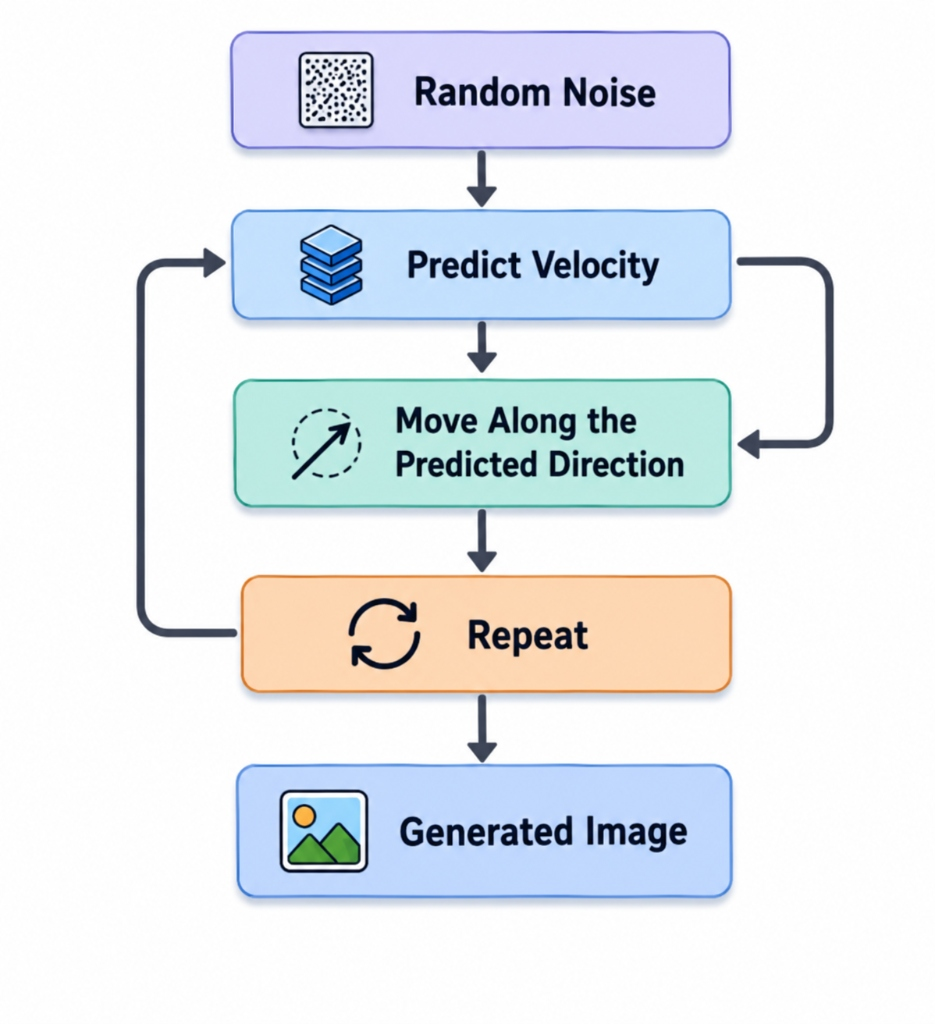
\includegraphics[width=0.65\textwidth]{figures/fig_10_12_flow_matching.jpg}
\caption{Flow Matching Denoising Loop.}
\label{fig:flow_matching}
\end{figure}

\subsection*{Advantages}
\begin{itemize}
    \item Simpler training objective
    \item Faster image generation with efficient ODE solvers
    \item Uses almost the same architecture as modern diffusion models
    \item Achieves state-of-the-art image generation quality.
\end{itemize}
